\documentclass{article}
\usepackage[utf8]{inputenc}
\usepackage{amsmath}
\usepackage{geometry}
\usepackage{multicol}
\usepackage{graphicx}
\usepackage{float}
\geometry{margin=1in}

\begin{document}

\newpage
\section*{Problema 1}





\textbf{Problema:} Se desea preparar 250 mL de una solución acuosa de Na$_2$CO$_3$ de concentración 21.50 g/L y densidad de 1.03 g/mL. \\
a) Calcula la masa de soluto que se deberá pesar. MM=126 g/mol, 1mol=2eq. g \\
b) Expresa la concentración en términos de: \% masa, fracción molar, molaridad y normalidad de la sal y de los respectivos iones.

\begin{multicols}{2} % Divide el contenido en dos columnas.
\noindent\textbf{Datos:} % Define la sección de datos en la columna izquierda.

\begin{figure}[H]
    \begin{minipage}[t]{0.3\textwidth} % Define un espacio del 30% del ancho del texto.
        \raggedright % Alinea a la izquierda dentro del minipage.
        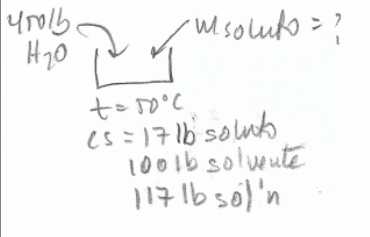
\includegraphics[width=\linewidth, height=2cm]{./problema1_diagrama.png} % Usa todo el ancho disponible en el minipage.
        \caption{Diagrama del \\ problema}
    \end{minipage}
\end{figure}

\textbf{} % Define las variables y fórmulas utilizadas en el problema.
\begin{itemize}
\item C = 21.50\% (concentración)
\item $\rho$ = 1.03 $\frac{g}{mL}$ (densidad)
\item V = 250 mL = 0.250 L (volumen de la solución)
\end{itemize}
\textbf{Cálculo del porcentaje en peso:}

\begin{align*}
    \%w &= \frac{5.375}{257.50} \times 100 = 2.08 \, \%
\end{align*}

\textbf{Cálculo de la fracción molar:}

\begin{align*}
    X_n &= \frac{4.266 \times 10^{-2} \, \text{mol}}{14.057 \, \text{mol}} = 3.036 \times 10^{-3}
\end{align*}

\textbf{Cálculo de la molaridad:}

\begin{align*}
    C &= 21.50 \, \% \times \frac{\frac{1 \, \text{mol}}{126 \, g}}{L} = 0.171 \, M
\end{align*}

\columnbreak % Indica el cambio a la columna derecha.

\noindent\textbf{Resolución:} % Define la sección para los incisos y la resolución del problema.

\textbf{a) Masa del soluto:}

\begin{align*}
    m_{\text{soluto}} &= 21.50 \, \% \times \frac{g}{100 \, g} \times 0.250 \, L = 5.375 \, g \, \text{soluto}
\end{align*}

\textbf{b) Masa de la solución:}

\begin{align*}
    m_{\text{soluto}} &= 250 \, mL \times \frac{1.03 \, g}{mL} = 257.50 \, g \, \text{solución} \\[10pt]
    m_{\text{solvente}} &= 257.50 - 5.375 = 252.125 \, g \, \text{solvente}
\end{align*}
\begin{align*}
    n_{\text{soluto}} &= 5.375 \, g \times \frac{1mol \, g}{126g} = 4.266x10^{-2} \,  \, \text{mol} \\[10pt]
    n_{\text{solvente}} &= 252.125g \times \frac{1mol \, g}{18g} = \frac{14.007mol \, g}{14.05mol}
\end{align*}


\textbf{Cálculo de la normalidad:}

\begin{align*}
    N &= 0.171 \, \frac{\text{mol}}{L} \times \frac{2 \, \text{eq}}{1 \, \text{mol}} = 0.342 \, \frac{\text{eq}}{L}
\end{align*}

\textbf{Reacción química:}

\begin{align*}
    \text{Na}_2\text{CO}_3 \rightarrow 2\text{Na}^+ + \text{CO}_3^{2-} \\
    \text{0.171M} \rightarrow \text{0.342M } \text{ 0.171M} \\
    \text{0.342M} \rightarrow \text{0.342M }\text{ 0.342M}
\end{align*}

\end{multicols} % Finaliza la división en dos columnas.









\newpage
\section*{Problema 2}
\textbf{Problema:} Se requiere preparar 1.500 L de solución acuosa de KMnO$_4$ de concentración 0.4 N, la cual será usada en una reacción redox en donde uno de los productos es Mn$^{2+}$. La sal con que se cuenta para la preparación contiene 10\% de impurezas insolubles. Calcula la masa de KMnO$_4$ impuro que se debe pesar y reporta la concentración en términos de molaridad, \% masa, molalidad, fracción mol y g/L.

\begin{multicols}{2} % Divide el contenido en dos columnas.
\noindent\textbf{Datos:} % Define la sección de datos en la columna izquierda.

\begin{figure}[H]
    \begin{minipage}[t]{0.3\textwidth} % Define un espacio del 30% del ancho del texto.
        \raggedright % Alinea a la izquierda dentro del minipage.
        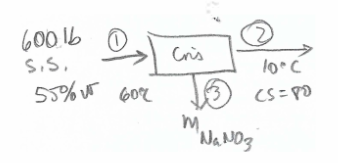
\includegraphics[width=\linewidth, height=2cm]{./problema2_diagrama.png} % Usa todo el ancho disponible en el minipage.
        \caption{Diagrama del \\ problema}
    \end{minipage}
\end{figure}

\textbf{} % Define las variables y fórmulas utilizadas en el problema.
\begin{itemize}
\item MM = 158 (Masa molar de KMnO$_4$)
\item V = 1.5 L (volumen de la solución)
\item C = 0.4 N (normalidad de la solución)
\item $\rho_{\text{sol}} = \rho_{\text{H}_2\text{O}} = 1 \frac{g}{mL}$ (densidad de la solución)
\item 10\% impurezas
\end{itemize}

\columnbreak % Indica el cambio a la columna derecha.

\noindent\textbf{Resolución:} % Define la sección para los incisos y la resolución del problema.

\textbf{Masa de impurezas:}

\begin{align*}
    M_{\text{impurezas}} &= 18.96 \, \text{g impuras} \times \frac{100 \, \text{g puras}}{90 \, \text{g impuras}} = 21.06 \, \text{g impuras}
\end{align*}

\textbf{Cálculo de la concentración (C):}

\begin{align*}
    C &= \frac{18.96 \, \text{g}}{1.5 \, \text{L}} = 12.64 \, \frac{\text{g}}{\text{L}}
\end{align*}

\textbf{Cálculo de la molaridad (M):}

\begin{align*}
    M &= \frac{0.12 \, \text{mol}}{1.5 \, \text{L}} = 0.08 \, \frac{\text{mol}}{\text{L}}
\end{align*}

\textbf{Cálculo del porcentaje en peso:}

\begin{align*}
    \%w &= \frac{18.96}{1500} \times 100 = 1.26 \, \%
\end{align*}

\textbf{Cálculo de la molalidad (m):}

\begin{align*}
    m &= \frac{0.12 \, \text{mol}}{1.481 \, \text{kg}} = 0.081 \, \frac{\text{mol}}{\text{kg}}
\end{align*}

\textbf{Cálculo de la fracción molar (X$_n$):}

\begin{align*}
    X_n &= \frac{0.12 \, \text{mol}}{82.40 \, \text{mol}} = 1.46 \times 10^{-3}
\end{align*}


\textbf{Masa de KMnO$_4$:}

\begin{align*}
    m_{\text{KMnO}_4} &= 0.4 \, \frac{\text{g}}{\text{L}} \times \frac{1 \, \text{mol}}{54 \, \text{g}} \times \frac{158 \, \text{g}}{1 \, \text{mol}} \times 1.5 \, \text{L} = 18.96 \, \text{g KMnO}_4
\end{align*}

\textbf{Cálculo de la masa de la solución:}

\begin{align*}
    m_{\text{solución}} &= 1500 \, \text{mL} \times \frac{1 \, \text{g}}{\text{mL}} = 1500 \, \text{g solución} \\[10pt]
    m_{\text{solvente}} &= 1500 - 18.96 = 1481.04 \, \text{g solvente} = 1.481 \, \text{kg}
\end{align*}

\textbf{Moles de soluto y solvente:}

\begin{align*}
    n_{\text{soluto}} &= \frac{18.96 \, \text{g}}{158 \, \text{g/mol}} = 0.12 \, \text{mol soluto} \\[10pt]
    n_{\text{solvente}} &= \frac{1481.04 \, \text{g}}{18 \, \text{g/mol}} = \frac{82.28\text{ mol solvente}}{82.40\text{ mol sol'n}} \,  \\[10pt]
\end{align*}

\end{multicols} % Finaliza la división en dos columnas.









\newpage
\section*{Problema 3}
\textbf{Problema:} Una solución se prepara a partir de 230 g de Pb(C$_2$H$_3$O$_2$)$_2$ • 3H$_2$O y 200 mL de agua destilada, la densidad que presenta la solución preparada se valora en 1.13 g/mL. Determina la concentración en términos de:
a) molalidad,
b) \% masa,
c) molaridad de la sal y de los iones,
d) normalidad de la sal y de los iones,
e) fracción mol.

\begin{multicols}{2} % Divide el contenido en dos columnas.
\noindent\textbf{Datos:} % Define la sección de datos en la columna izquierda.

\begin{figure}[H]
    \begin{minipage}[t]{0.3\textwidth} % Define un espacio del 30% del ancho del texto.
        \raggedright % Alinea a la izquierda dentro del minipage.
        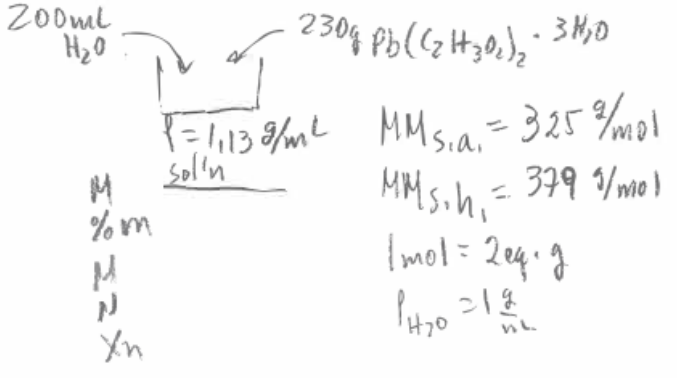
\includegraphics[width=\linewidth, height=2cm]{./problema3_diagrama.png} % Usa todo el ancho disponible en el minipage.
        \caption{Diagrama del \\ problema}
    \end{minipage}
\end{figure}

\textbf{} % Define las variables y fórmulas utilizadas en el problema.
\begin{itemize}
\item V = 200 mL de agua
\item m$_{\text{soluto}}$ = 230 g de Pb(C$_2$H$_3$O$_2$)$_2 \cdot$ 3H$_2$O
\item $\rho_{\text{solución}}$ = 1.13 g/mL
\item MM$_{\text{s.a.}}$ = 325 g/mol (masa molar del soluto anhidro)
\item MM$_{\text{s.h.}}$ = 379 g/mol (masa molar del soluto hidratado)
\item 1 mol = 2 eq (equivalentes)
\item $\rho_{\text{H}_2\text{O}}$ = 1 g/mL
\end{itemize}

\columnbreak % Indica el cambio a la columna derecha.

\noindent\textbf{Resolución:} % Define la sección para los incisos y la resolución del problema.

\textbf{Cálculo de masas:}

\begin{align*}
    m_{\text{soluto}} &= 230g s.h \frac{325sa}{379sh}=197.23g  s.a\\
    m_{\text{sol'n}} &= 230 \, \text{g s.h.} + 200 \, \text{g H}_2\text{O} = 430 \, \text{g solución} \\[10pt]
    m_{\text{solvente}} &= 430 - 197.23 = 232.77 \, \text{g solvente} = 0.233 \, \text{kg H}_2\text{O}
\end{align*}

\textbf{Moles de soluto:}

\begin{align*}
    n_{\text{soluto}} &= \frac{197.23 \, \text{g}}{325 \, \text{g/mol}} = 0.607 \, \text{mol soluto}
\end{align*}

\textbf{Moles de solvente:}

\begin{align*}
    n_{\text{solvente}} &= 232.77 \, \text{g H}_2\text{O} \times \frac{1 \, \text{mol}}{18 \, \text{g}} = 12.932 \, \text{mol}
\end{align*}

\textbf{Total de moles de solución:}

\begin{align*}
    n_{\text{solución}} &= 0.607 + 12.932 = 13.539 \, \text{mol}
\end{align*}

\textbf{a) Molalidad (m):}

\begin{align*}
    m &= \frac{0.607 \, \text{mol}}{0.233 \, \text{kg}} = 2.605 \, \frac{\text{mol}}{\text{kg}}
\end{align*}

\textbf{b) Porcentaje en masa:}

\begin{align*}
    \% \text{masa} &= \frac{197.23 \, \text{g}}{430 \, \text{g}} \times 100 = 45.9\%
\end{align*}

\textbf{c) Fracción molar (X$_n$):}

\begin{align*}
    X_n &= \frac{0.607 \, \text{mol}}{13.539 \, \text{mol}} = 0.045
\end{align*}

\textbf{Volumen de la solución:}

\begin{align*}
    V_{\text{solución}} &= \frac{430 \, \text{g solución}}{1.13 \, \text{g/mL}} = 380.53 \, \text{mL} = 0.381 \, \text{L}
\end{align*}

\textbf{d) Molaridad (M):}
\begin{align*}
    M &= \frac{0.607 \, \text{mol}}{0.381 \, \text{L}} = 1.593 \, \frac{\text{mol}}{\text{L}}
\end{align*}

\textbf{e) Normalidad (N):}

\begin{align*}
    N &= 1.593 \, \frac{\text{mol}}{\text{L}} \times \frac{2 \, \text{eq}}{1 \, \text{mol}} = 3.186 \, \frac{\text{eq}}{\text{L}}
\end{align*}

\textbf{Reacción química:}
\begin{align*}
    \text{Pb(C}_2\text{H}_3\text{O}_2\text{)}_2 \rightarrow \text{Pb}^{+2} + 2\text{C}_2\text{H}_3\text{O}_2^{-} \\
    c) \hspace{0.5cm} \text{1.593M} \rightarrow \text{1.593M } \text{1.593M} \\
    d) \hspace{0.8cm} \text{3.186N} \rightarrow \text{3.186N} \text{3.186N}
\end{align*}

\textbf{Concentraciones finales:}

\begin{align*}
    \text{Pb}^{+2} &: 1.593 \, M, \, 3.186 \, N \\[10pt]
    \text{C}_2\text{H}_3\text{O}_2^{-} &: 3.186 \, M, \, 3.186 \, N
\end{align*}

\end{multicols} % Finaliza la división en dos columnas.









\newpage
\section*{Problema 4}
\textbf{Problema:} Una solución de H$_2$SO$_4$ tiene una concentración 10.5 \% masa y densidad ($\rho$) = 1.07 g/mL. Expresa la concentración en términos de normalidad y molaridad cuando dicha solución interviene en una reacción cuyo producto es H$_2$S.

\begin{multicols}{2} % Divide el contenido en dos columnas.
\noindent\textbf{Datos:} % Define la sección de datos en la columna izquierda.

\begin{figure}[H]
    \begin{minipage}[t]{0.3\textwidth} % Define un espacio del 30% del ancho del texto.
        \raggedright % Alinea a la izquierda dentro del minipage.
        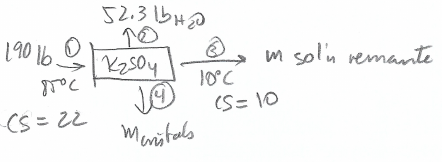
\includegraphics[width=\linewidth, height=2cm]{./problema4_diagrama.png} % Usa todo el ancho disponible en el minipage.
        \caption{Diagrama del \\ problema}
    \end{minipage}
\end{figure}

\textbf{} % Define las variables y fórmulas utilizadas en el problema.
\begin{itemize}
\item MM = 98 g/mol (masa molar de H$_2$SO$_4$)
\item C = 10.5\% w/v (concentración en peso por volumen)
\item $\rho$ = 1.07 g/mL (densidad de la solución)
\item N = ? (normalidad)
\item M = ? (molaridad)
\item 1 mol = 8 eq (equivalentes)
\end{itemize}

\columnbreak % Indica el cambio a la columna derecha.

\noindent\textbf{Resolución:} % Define la sección para los incisos y la resolución del problema.

\textbf{Cálculo de la concentración en g/L:}

\begin{align*}
    C &= \frac{10.5 \, \text{g soluto}}{100 \, \text{g solución}} \times \frac{1.07 \, \text{g solución}}{\text{mL solución}} \times \frac{1000 \, \text{mL solución}}{1 \, \text{L solución}} \\[10pt]
    C &= 112.35 \, \frac{\text{g}}{\text{L}}
\end{align*}

\textbf{Cálculo de la molaridad (M):}

\begin{align*}
    M &= \frac{112.35 \, \text{g/L}}{98 \, \text{g/mol}} = 1.146 \, \frac{\text{mol}}{\text{L}}
\end{align*}

\textbf{Cálculo de la normalidad (N):}

\begin{align*}
    N &= 1.146 \, \frac{\text{mol}}{\text{L}} \times \frac{8 \, \text{eq}}{1 \, \text{mol}} = 9.168 \, \frac{\text{eq}}{\text{L}}
\end{align*}

\textbf{Reacción de H$_2$SO$_4$:}

\begin{align*}
    \text{H}_2\text{SO}_4 + 8e^- \rightarrow \text{H}_2\text{S}^{-2} %+ 4\text{H}_2\text{O}
\end{align*}

\end{multicols} % Finaliza la división en dos columnas.









\newpage
\section*{Problema 5}
\textbf{Problema:} Determina la masa de Na$_3$PO$_4$ que debe disolverse en 500 mL de solución, a fin de que la solución preparada presente una concentración de 0.15 mol/L. Expresa la concentración en términos de normalidad (N), \% en peso (\%w), fracción molar (X$_n$), molalidad (m) y g/L.

\begin{multicols}{2} % Divide el contenido en dos columnas.
\noindent\textbf{Datos:} % Define la sección de datos en la columna izquierda.

\begin{figure}[H]
    \begin{minipage}[t]{0.3\textwidth} % Define un espacio del 30% del ancho del texto.
        \raggedright % Alinea a la izquierda dentro del minipage.
        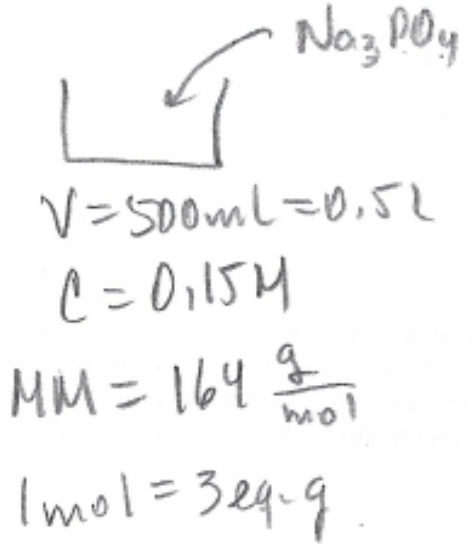
\includegraphics[width=\linewidth, height=2cm]{./problema5_diagrama.png} % Usa todo el ancho disponible en el minipage.
        \caption{Diagrama del \\ problema}
    \end{minipage}
\end{figure}

\textbf{} % Define las variables y fórmulas utilizadas en el problema.
\begin{itemize}
\item V = 500 mL = 0.5 L (volumen de la solución)
\item C = 0.15 M (molaridad)
\item MM = 164 g/mol (masa molar de Na$_3$PO$_4$)
\item 1 mol = 3 eq (equivalentes)
\item Supuesto: $\rho_{\text{solución}} = \rho_{\text{H}_2\text{O}} = 1 \frac{g}{mL}$ (densidad)
\end{itemize}

\columnbreak % Indica el cambio a la columna derecha.

\noindent\textbf{Resolución:} % Define la sección para los incisos y la resolución del problema.

\textbf{Masa del soluto:}

\begin{align*}
    m_{\text{soluto}} &= 0.15 \, \frac{\text{mol}}{\text{L}} \times 0.5 \, \text{L} \times 164 \, \frac{\text{g}}{\text{mol}} = 12.30 \, \text{g soluto}
\end{align*}

\textbf{Masa de la solución:}

\begin{align*}
    m_{\text{solución}} &= 500 \, \text{mL} \times \frac{1 \, \text{g}}{\text{mL}} = 500 \, \text{g solución}
\end{align*}

\textbf{Masa del solvente:}

\begin{align*}
    m_{\text{solvente}} &= 500 \, \text{g} - 12.30 \, \text{g} = 487.70 \, \text{g solvente} = 0.488 \, \text{kg}
\end{align*}

\textbf{Moles de soluto y solvente:}

\begin{align*}
    n_{\text{soluto}} &= \frac{12.30 \, \text{g}}{164 \, \frac{\text{g}}{\text{mol}}} = 0.075 \, \text{mol soluto} \\[10pt]
    n_{\text{solvente}} &= 487.70 \, \text{g} \times \frac{1 \, \text{mol}}{18 \, \text{g}} = 27.094 \, \text{mol solvente} \\[10pt]
    n_{\text{solución}} &= 0.075 + 27.094 = 27.169 \, \text{mol}
\end{align*}

\textbf{a) Normalidad (N):}

\begin{align*}
    N &= 0.15 \, \frac{\text{mol}}{\text{L}} \times \frac{3 \, \text{eq}}{1 \, \text{mol}} = 0.45 \, \frac{\text{eq}}{\text{L}}
\end{align*}

\textbf{b) Porcentaje en peso (\%w):}

\begin{align*}
    \%w &= \frac{12.30 \, \text{g}}{500 \, \text{g}} \times 100 = 2.46 \, \%
\end{align*}

\textbf{c) Fracción molar (X$_n$):}

\begin{align*}
    X_n &= \frac{0.075 \, \text{mol}}{27.169 \, \text{mol}} = 2.76 \times 10^{-3}
\end{align*}

\textbf{d) Molalidad (m):}

\begin{align*}
    m &= \frac{0.075 \, \text{mol}}{0.488 \, \text{kg}} = 0.154 \, \frac{\text{mol}}{\text{kg}}
\end{align*}

\textbf{e) Concentración (C):}

\begin{align*}
    C &= \frac{12.30 \, \text{g}}{0.5 \, \text{L}} = 24.60 \, \frac{\text{g}}{\text{L}}
\end{align*}

\end{multicols} % Finaliza la división en dos columnas.









\newpage
\section*{Problema 6}
\textbf{Problema:}
Se requiere una solución 0.45 N de fosfato plúmbico Pb$_3$(PO$_4$)$_4$. Determinar la masa de soluto y solvente necesaria y expresar la concentración en términos de: \% masa, fracción mol, molalidad, g/L y molaridad. Considerar una densidad de solución igual a 1.08 g/mL.

\begin{multicols}{2} % Divide el contenido en dos columnas.
\noindent\textbf{Datos:} % Define la sección de datos en la columna izquierda.

\begin{figure}[H]
    \begin{minipage}[t]{0.3\textwidth} % Define un espacio del 30% del ancho del texto.
        \raggedright % Alinea a la izquierda dentro del minipage.
        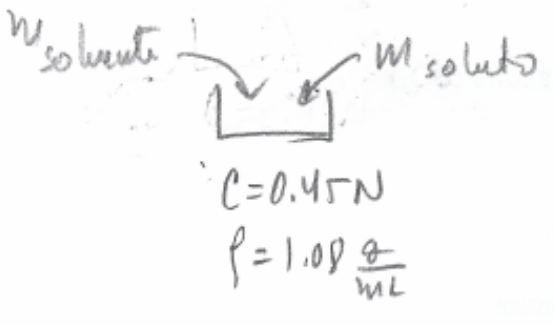
\includegraphics[width=\linewidth, height=2cm]{./problema6_diagrama.png} % Usa todo el ancho disponible en el minipage.
        \caption{Diagrama del \\ problema}
    \end{minipage}
\end{figure}

\textbf{} % Define las variables y fórmulas utilizadas en el problema.
\begin{itemize}
\item C = 0.45 N (normalidad de la solución)
\item $\rho$ = 1.08 g/mL (densidad de la solución)
\item MM = 1001 g/mol (masa molar de Pb$_3$(PO$_4$)$_4$)
\item 1 mol = 12 eq (equivalentes)
\item Base de cálculo: 1 L de solución
\end{itemize}

\columnbreak % Indica el cambio a la columna derecha.

\noindent\textbf{Resolución:} % Define la sección para los incisos y la resolución del problema.

\textbf{Masa del soluto:}

\begin{align*}
    m_{\text{soluto}} &= 0.45 \, \frac{\text{eq}}{\text{L}} \times 1 \, \text{L} \times \frac{1 \, \text{mol}}{12 \, \text{eq}} \times \frac{1001 \, \text{g}}{1 \, \text{mol}} = 37.538 \, \text{g Pb}_3(\text{PO}_4)_4
\end{align*}

\textbf{Masa del solvente:}

\begin{align*}
    m_{\text{solvente}} &= 1080 \, \text{g solución} - 37.538 \, \text{g soluto} \\
    &= 1042.462 \, \text{g H}_2\text{O} = 1.042 \, \text{kg}
\end{align*}

\textbf{Moles de soluto y solvente:}

\begin{align*}
    n_{\text{soluto}} &= \frac{37.538 \, \text{g}}{1001 \, \text{g/mol}} = 0.036 \, \text{mol soluto} \\[10pt]
    n_{\text{solvente}} &= 1042.462 \, \text{g} \times \frac{1 \, \text{mol}}{18 \, \text{g}} = 57.915 \, \text{mol solvente}
\end{align*}

\textbf{Total de moles de solución:}

\begin{align*}
    n_{\text{solución}} &= 0.036 \, \text{mol} + 57.915 \, \text{mol} = 57.951 \, \text{mol soln}
\end{align*}

\textbf{a) Porcentaje en masa (\%m):}

\begin{align*}
    \%m &= \frac{37.538 \, \text{g soluto}}{1080 \, \text{g solución}} \times 100 = 3.48 \, \%
\end{align*}

\textbf{b) Molalidad (m):}

\begin{align*}
    m &= \frac{0.036 \, \text{mol}}{1.042 \, \text{kg H}_2\text{O}} = 0.035 \, \frac{\text{mol}}{\text{kg}}
\end{align*}

\textbf{c) Fracción molar (X$_n$):}

\begin{align*}
    X_n &= \frac{0.036 \, \text{mol}}{57.951 \, \text{mol}} = 0.001
\end{align*}

\textbf{d) Molaridad (M):}

\begin{align*}
    M &= \frac{0.036 \, \text{mol}}{1 \, \text{L}} = 0.036 \, \text{M}
\end{align*}

\textbf{e) Concentración en g/L (C):}

\begin{align*}
    C &= \frac{37.538 \, \text{g}}{1 \, \text{L}} = 37.538 \, \frac{\text{g}}{\text{L}}
\end{align*}

\end{multicols} % Finaliza la división en dos columnas.

\end{document}